\documentclass{article}
\title{CSCI 2200 HW1}
\author{Xinshi,Wang}
\usepackage[letterpaper,textwidth=5.5in,right=0.6in,textheight=9in,left=0.6in,top=0.7in,bottom=0.7in]{geometry}
\usepackage{scrextend}
\usepackage{graphicx}
\usepackage{xcolor}
\usepackage{amssymb}
\begin{document}
\noindent
CSCI 2200 HW1\\
Wang Xinshi\\

%Q (1.21) starts from here
\noindent Q (1.21) A building has 1000 floors. You wish to determine the highest floor from which you can drop an egg without the egg breaking. If you had 1000 identical eggs, you could drop one from each floor and see which eggs survive. How many egg drop trials do you need if you have: (a) One egg. (b) Two identical eggs.\\

\textcolor{blue}{
\begin{addmargin}[2em]{2em}
	\quad I need at most 1000 trials if I have one egg. I will need to drop it from the first floor, and increase the floor level one by one until it cracks, so it at most takes 1000 trails.
\end{addmargin}}
	
\textcolor{blue}{
	\begin{addmargin}[2em]{2em}
		\quad I need at most 45 trials if I have two identical eggs. Label those two eggs egg1 and egg2. Firstly, drop egg1 from floor n. If it cracks, then start dropping egg2 from the $1^{st}$ floor until the $n^{th}$ floor to see which floor it cracks. If it did not crack, then go $n-1$ floors up and drop it again. repeat the process until it cracks, and then use egg2 to test each floor in this interval. Then the increment on the floor levels from the initial drop is $n+(n-1)+(n-2)+... = \frac{n(n+1)}{2}.$ Therefore, to test 1000 floors, it takes $\frac{n(n+1)}{2} = 1000$, which is $n = 44.2 \approx 45 trails$ if we initially drop it from the $45^{th}$ floor. 
	\end{addmargin}}
%Q (1.21) ends here
\clearpage

%Q (1.32) starts from here
\noindent Q (1.32) 25 horses have different speeds. You can race up to 5 horses at a time and observe the order in which the horses finish. You have no stop-watch. Show that 7 races suffice to determine the fastest 3 horses.

\begin{table}[h]
	\center
	\caption{\textcolor{blue}{Divide the horses into $5$ groups, rank them from slowest to fastest}}
	\textcolor{blue}{
	\begin{tabular}{| c | c | c | c | c |}
		\hline
		$5^{th}$ place & $4^{th}$  place & $3^{rd}$  place & $2^{nd}$  place & $1^{st}$  place\\ 
		\hline
		$g_{11}$&$g_{12}$&$g_{13}$&$g_{14}$&$g_{15}$\\
		\hline
		$g_{21}$&$g_{22}$&$g_{23}$&$g_{24}$&$g_{25}$\\
		\hline
		$g_{31}$&$g_{32}$&$g_{33}$&$g_{34}$&$g_{35}$\\
		\hline
		$g_{41}$&$g_{42}$&$g_{43}$&$g_{44}$&$g_{45}$\\
		\hline
		$g_{51}$&$g_{52}$&$g_{53}$&$g_{54}$&$g_{55}$\\
		\hline
	\end{tabular}}
\end{table}

\begin{addmargin}[2em]{2em}
	\textcolor{blue}{
	\quad Firstly, divide the 25 hourses into 5 groups and race them group by group gives us the champions for each group, which are $g_{15}$, $g_{25}$, $g_{35}$, $g_{45}$, and $g_{55}$.}

	\textcolor{blue}{
 Next, we race the $5$ champions in another round, which will give us a rank between these $5$ horses. Let us assume that $g_{15}$ is the fastest and $g_{55}$ is the slowest, and other horses follow the same rule. Up until this point, we have used 6 races, and we can eliminate some horses so we are left with $5$ horses to do the last round.\\
}
\textcolor{blue}{
  \quad We know that to there can not be 3 or more horses that are faster than the top three horses, so we can eliminate all the horses in $g_5$ because horses from $g_{51}$ to $g_{54}$ are all slower than $g_{55}$ and $g_{55}$ was the last in the final round. We can also eliminate $g_4$ for the same reason. we can also eliminate horses from $g_{31}$ to $g_{34}$ since $g_{35}$ is the third place in the last round. The same reason could be applied to horses from $g_{21}$ to $g_{23}$ and horses from $g_{11}$ to $g_{12}$.
We can eliminate $g_{15}$ since it is the champion. Then, we are left with exactly five horses to do the last round, which are $g_{35}$, $g_{24}$, $g_{25}$, $g_{13}$, and $g_{14}$. The $1^{st}$ place and the $2^{nd}$ place from the last round are the $2^{nd}$ and $3^{rd}$ in the race. Thus, we can rank the top three in 7 races.}
\end{addmargin}
%Q (1.32) ends here

\clearpage

%Q (2.5(d)) starts from here
\noindent Q (2.5(d) )Express the shaded regions using intersections, unions, and complements.
\begin{figure}[h]
	\centering
	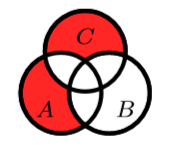
\includegraphics{"C:/Users/Micha/OneDrive - Rensselaer Polytechnic Institute/CSCI 2200/Latex_pictures/sets.png"}
\end{figure}
\\
\textcolor{blue}{
\indent First, let us represent the triangular-like region in the middlle, which is the intersection of three sets - $A \cap B \cap C$
	We can substract B by saying $(A \cup C) \cap B^c$. To eliminate the blank between $A$ and $C$, we need to substract the intersection between $A$ and $C$. However, the triangular-like section has already been counted. Therefore, the middle part between $A$ and $C$ should be represented as $A \cap C \cap (A \cap B \cap C)$}
	
	\textcolor{blue}{
	Therefore, the answer is $(A \cup C) \cap B^c \cap (A \cap C \cap (A \cap B \cap C)^c)^c$}
%Q (2.5(d)) ends here

\clearpage

%Q (2.21) starts from here%
\begin{addmargin}[2em]{2em}
	\indent Q (2.21) Express the following sequence using f(n), where n = 0,1,2,3,..., and then formally define the set of numbers.
	\begin{center}
		$0,1,-2,3,-4,5,-6,7...$
	\end{center}
	\textcolor{blue}{
		\indent We can see that the sign of the numbers in the squence is alternating, so there should be a coefficience $-1^{n+1}$ in front of the numbers in the sequence.}
	
	\textcolor{blue}{
		 The sequence follows the same pattern as non-negative real number sequence, so the $n^{th}$ term could be generalized as $S_n = f(n) = (-1)^{n+1}n$
	To represent it as a set, we could use}
	\begin{center}
		\textcolor{blue}{
			$A = \{a| a = 0$ or $a = (-1)^{n+1} \cdot n, n \in \mathbb{N}\}$}
	\end{center}
\end{addmargin}
%Q (2.21) ends here%

\clearpage
%Q (2.26) starts from here
\begin{addmargin}[2em]{0em}
	\indent Q (2.26) True or false and why? Every square which is a multiple of 4 came from a multiple of 4 and every multiple of 4 has a square which is a multiple of 4.
	
	\textcolor{blue}{The first part of the sentence is false. Let us assume there exists a square number $4k^2$ which is a multiple of 4. Then the squre root of the square number is $\sqrt{4k^2}$, which is $2k^2$. Therefore a square number that is a multiple of $4$ might come from a number that is a multiple of $2$. The second part of the claim is true. A number that i multiple of $4$ can be represented as 4k, and its square is $16k^2$, which is still a multiple of $4$.}
\end{addmargin}
%Q (2.26) ends here
\end{document}